\begin{figure}[h]
    \centering
    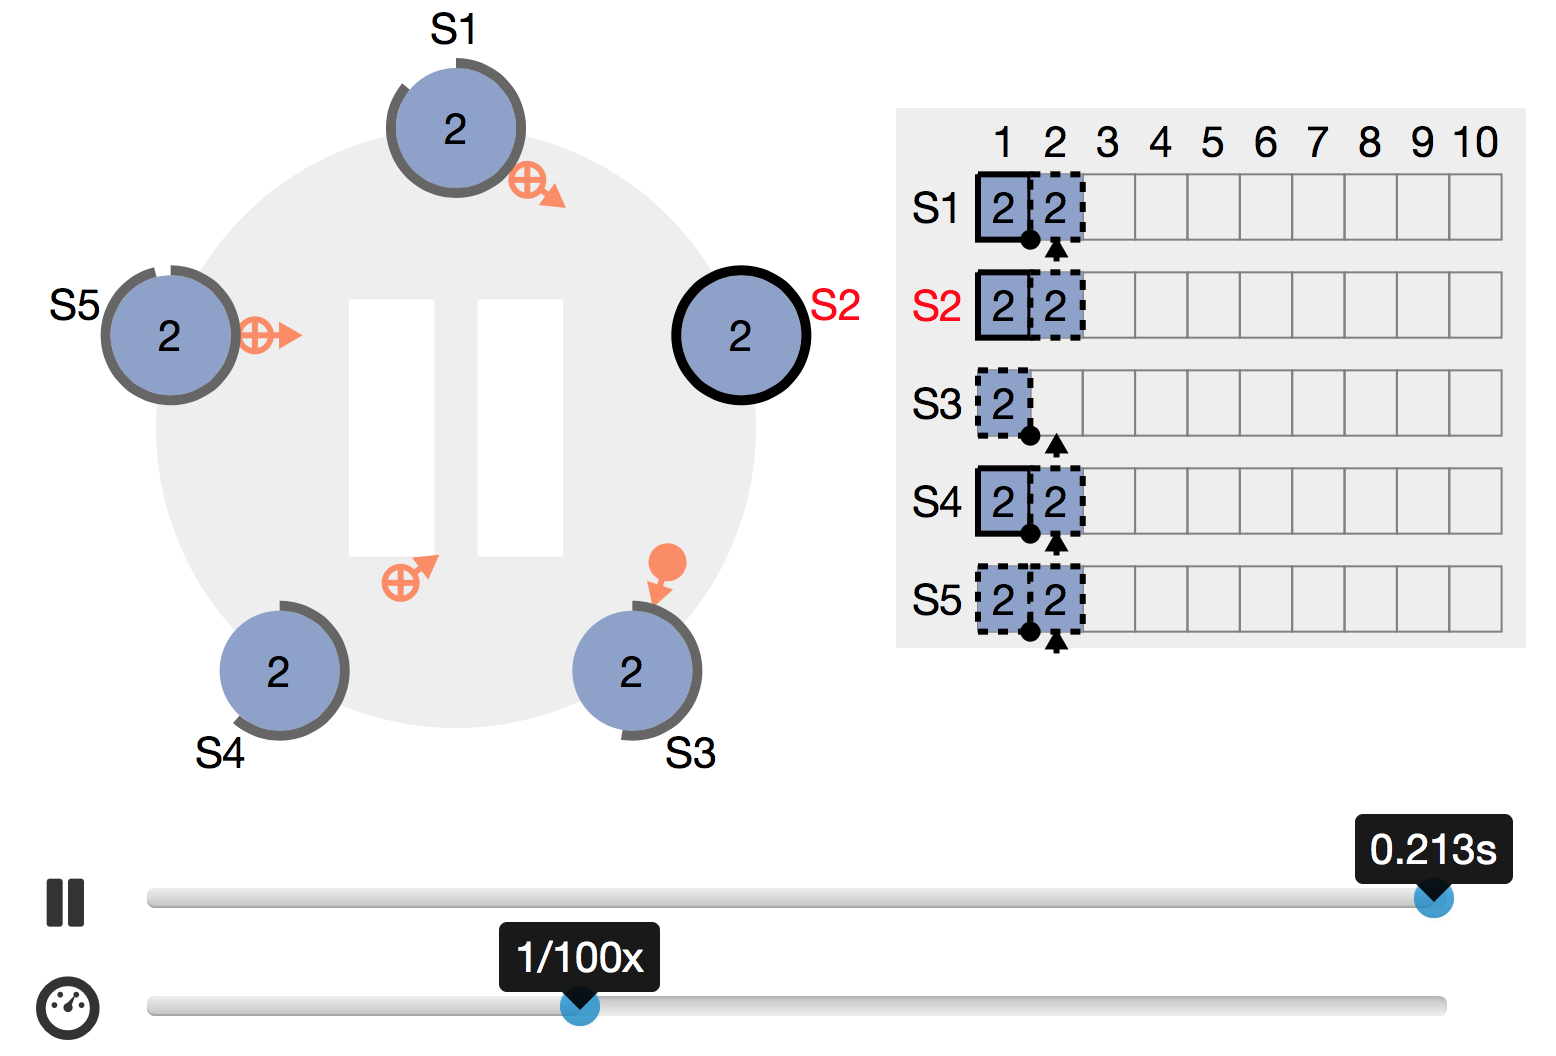
\includegraphics[width=0.9\linewidth]{org.png}
    \caption{Original}\label{fig:original}
\end{figure}
\subsection{Simulation model}

Raft Scope simulates a small Raft cluster in your browser. The user can pause the simulation, seek points in time and modify its speed.
It is coded in JavaScript, which is a single threaded language.
The author created a sort of virtual machine (VM) where
concurrency is only simulated by artificially managing time and events.

The VM has an internal clock that is advanced at each simulation cycle
by an amount of time computed \textit{w.r.t} the simulation speed.
For each simulation cycle, the main loop (\texttt{raft.update}) checks each server and loops through their
actions in a predefined order. If the simulated time advances past the timeout for the respective action, then
that event is fired in this cycle. In the same fashion the simulation loops through each message and delivers it if its
\texttt{DeliveryTime} has elapsed.

Due to this design decision and especially at very high simulation speeds (\textit{e.g.} real time speed)
many operations are executed in \emph{bulk} in the same cycle.
This does not guarantee correctness because the operations take place in their internal cycle ordering instead of
being ordered by their timeouts.

For example:
Suppose the cluster leader sends an \texttt{AppendEntries} message (M1)
to server 2~(S2), and that the S2 \texttt{ElectionTimeout} is due to expire just after
the arrival of M1. If the simulation speed is sufficiently high, it is possible that these two events
take place in the same simulation cycle, thus S2 would start an election because this event check happens before the
loop that delivers the messages.
In a real world application S2 would receive M1, reset its \texttt{ElectionTimeout}, and reply with the \texttt{ACK} message.

\subsection{Interaction}
The user can interact with the Raft cluster by sending \emph{client requests}, starting/stopping/restarting a server,
forcing a server to start a new election and dropping messages.
Each of these actions generates a new state in the simulation.
The user can save snapshots of a particular simulation and all of its checkpoints and replay it.

\subsection{Code organization}
The Raft Scope code base is organized mainly in three different files:
\begin{itemize}
\item \texttt{state.js}
\item \texttt{raft.js}
\item \texttt{script.js}
\end{itemize}

\texttt{state.js} manages the state of the simulation and keeps track of its configuration and its entities(servers,
messages, logs, etc...).
For each simulation cycle, the previous state is appended to a list of checkpoints and a new one is generated. This allows
the user to rewind and playback the simulation by jumping to a previous state.

\texttt{raft.js} manages the rules of the simulation. Rules are actions defined by the protocol,
such as \textit{BecomeLeader}, \textit{StartNewElection}, \textit{SendRPC}, etc... These are connected to the time of the simulation and are checked
automatically by the main loop.

\texttt{script.js} handles everything else: connecting entities to their graphical representation, generating the log table,
 initializing the simulation. This code was particularily tricky to understand at first.
